\section{Simulações}

\subsection{Circuito amplificador-diferenciador}

\subsubsection{Diferenciador Senoidal}

\textbf{a)} Simule o circuito da Figura 1 para $R_c=0$ e para $R_c=100\ohm$. Utilize $R = 1k\ohm$ e $C = 1\mu F$. Verifique a saída $V_{out}(t)$ para $V_{in}(t)$ ajustado em $2V_{pp}$ e $100 Hz$ nos seguintes formatos: senoidal, quadrada e triangular.

\begin{itemize}
    \item Na aba Componentes, vá em componentes nãolineares e coloque um Amplificador Operacional. Vá em componentes agrupados e coloque dois resistores e um capacitor. Vá em Fontes e coloque uma fonte de tensão AC. Vá em Ponteiras e coloque uma ponteira de tensão.
\end{itemize}

\begin{figure}[H]
    \subfiguras{.20}{1}{imagens/diferenciador_senoidal/opamp_sel}{}{}
    \subfiguras{.20}{1}{imagens/diferenciador_senoidal/probes}{}{}
    \subfiguras{.20}{1}{imagens/diferenciador_senoidal/cap_resis}{}{}
    \subfiguras{.20}{1}{imagens/diferenciador_senoidal/ac_voltage}{}{}
\end{figure}


\begin{itemize}
    \item Conecte os componentes sem esquecer da referência do terra e ajuste seus valores para os pedidos no exercício. Nomeie o nó de saída.
\end{itemize}

\figuras{.5}{imagens/diferenciador_senoidal/circuito_diferenciador.png}{Circuito Diferenciador.}{circ_diff}
    
\begin{itemize}
    \item Será utilizada a simulação transiente para se observar o comportamento do circuito ao longo do tempo. O período da onda é de 10ms.
\end{itemize}

\figuras{.4}{imagens/diferenciador_senoidal/sim_transiente}{Simulação Transiente.}{sim_trans}

\begin{itemize}
    \item Salve e simule o circuito.
\end{itemize}

\figuras{1}{imagens/diferenciador_senoidal/sal_sim}{}{}

\begin{itemize}
    \item Vá em Diagramas e insira uma tabela. Coloque o valor da tensão $V_o$.\textsc{v}.
\end{itemize}

\figuras{.5}{imagens/diferenciador_senoidal/diagram}{Inserção dos valores do Gráfico}{}

\begin{itemize}
    \item E assim verifica-se os valores pedidos no exercício.
\end{itemize}

\figuras{.5}{imagens/diferenciador_senoidal/final}{Forma de onda exigida no exercício.}{}

\begin{itemize}
    \item Para $R_c=100\ohm$, ajuste o valor do resistor, salve e simule. O gráfico deve estar na seguinte forma.
\end{itemize}

\figuras{.5}{imagens/diferenciador_senoidal/final_R_100.png}{Circuito com $R_c=100$.}{}

\newpage

\subsubsection{Diferenciador Quadrado}

\begin{itemize}
    \item Vá em Arquivo $\rightarrow$Salvar como... e mude o nome do arquivo para utilizar o esquemático para o próximo circuito. Na aba Componentes, vá em Fontes e coloque uma fonte de tensão retangular e uma fonte DC. Apague a fonte de tensão AC.
\end{itemize}

\begin{figure}[H]
    \centering
    \subfiguras{.25}{1}{imagens/diferenciador_quadrado/source_square}{}{}
    \subfiguras{.25}{1}{imagens/diferenciador_quadrado/dc_voltage}{}{}
\end{figure}


\begin{itemize}
    \item Queremos uma onda quadrada, logo U deve ser $2V$.
    Como a frequência é de 100 Hz, $T_H$ e $T_L$ devem ser 5
    ms. $T_r$ e $T_f$ devem ser igual a zero, pois a mudança de
    nível é instantânea.
\end{itemize}

\figuras{.5}{imagens/diferenciador_quadrado/edit_square_wave}{Parâmetros para onda quadrada.}{}

\begin{itemize}
    \item Para deslocar a onda na metade da amplitude e
    colocar para ela variar entre +1V e –1V, será utilizada
    uma fonte DC de -1V. Conecte os componentes sem
    esquecer da referência do terra e ajuste seus valores
    para os pedidos no exercício. Nomeie o nó de saída.
\end{itemize}

\figuras{.5}{imagens/diferenciador_quadrado/circuito}{Circuito montado no Qucs.}{}

\begin{itemize}
    \item Como o período da onda é de 10ms, coloque tempo
    suficiente para visualizar o comportamento da onda
    e resolução grande o suficiente para gerar a onda.
\end{itemize}

\figuras{.4}{imagens/diferenciador_quadrado/transient_sim}{Parâmetros para a simulação transiente.}{}

\begin{itemize}
    \item Salve e simule. Vá em Diagramas e insira um plano
    cartesiano. Coloque o valor das tensões Vo.Vt e
    Vin.Vt. Para visualizar a amplitude de Vo.Vt, coloque
    seu eixo y à direita.
\end{itemize}

\figura{1}{imagens/diferenciador_quadrado/save_sim}

\figuras{.4}{imagens/diferenciador_quadrado/diagram_edit}{Parâmetros para obtenção do diagrama.}{}


\begin{itemize}
    \item Assim, verifica-se que os valores pedidos no exercício.
\end{itemize}

\figuras{.5}{imagens/diferenciador_quadrado/final_R_0}{Comportamento do circuito exigido pelo exercício.}{}

\begin{itemize}
    \item Para $R_C=100\ohm$, ajuste o valor do resistor, salve e
    simule.
\end{itemize}

\figuras{.5}{imagens/diferenciador_quadrado/final_R_0}{Comportamento do circuito com $R_c=100\ohm$}{}

\subsubsection{Diferenciador Triângular}

\begin{itemize}
    \item Vá em Arquivo $\rightarrow$ Salvar como... e mude o nome do
    arquivo para utilizar o esquemático para o próximo
    circuito. Queremos uma onda triangular, logo U deve
    ser 2V. Como a frequência é de 100 Hz, encontra-se
    o valor do período de aproximadamente 10 ms, logo
    o valor do $T_H$, $T_L$, $T_r$ e $T_f$ devem ser 5 ms.
\end{itemize}


\figuras{.4}{imagens/diferenciador_triangular/source_edit}{Edição da fonte retangular para uma triangular.}{}

\begin{itemize}
    \item Para deslocar a onda na metade da amplitude e
    colocar para ela variar entre +1V e –1V, será utilizada
    uma fonte DC de -1V. Conecte os componentes sem
    esquecer da referência do terra e ajuste seus valores
    para os pedidos no exercício. Nomeie o nó de saída.
\end{itemize}

\figuras{.5}{imagens/diferenciador_triangular/circuito}{Circuito exigido pelo exercício.}{}

\begin{itemize}
    \item Como o período da onda é de 10ms, coloque tempo
    suficiente para visualizar o comportamento da onda
    e resolução grande o suficiente para gerar a onda.
\end{itemize}

\figuras{.4}{imagens/diferenciador_triangular/transient_sim}{Parâmetros para a simulação transiente.}{}

\begin{itemize}
    \item  Salve e simule. Vá em Diagramas e insira um plano
    cartesiano. Coloque o valor das tensões Vo.Vt e
    Vin.Vt. Para visualizar a amplitude de Vo.Vt, coloque
    seu eixo y à direita.
\end{itemize}

\figura{1}{imagens/diferenciador_triangular/save_sim}
\figuras{.5}{imagens/diferenciador_triangular/edit_diagram}{Edição dos eixos que compõem o gráfico.}{}


\begin{itemize}
    \item Assim, verifica-se os valores pedidos no exercício.
\end{itemize}
 
\figuras{.5}{imagens/diferenciador_triangular/final_R_0}{Comportamento do circuito exigido pelo exercício.}{}

\begin{itemize}
    \item Para $R_c=100\ohm$, ajuste o valor do resistor, salve e simule.
\end{itemize}

\figuras{.5}{imagens/diferenciador_triangular/final_R_100}{Comportamento do circuito com $R_c=100\ohm$}{}

\subsubsection{Circuito amplificador-integrador}

\subsubsection{Integrador Senoidal}

\begin{itemize}
    \item Simule o circuito da Figura 2 para $R_o \rightarrow \infty$ e para
    $R_o=100\ohm$. Utilize $R=1k\ohm$ e $C=1\mu F$. Verifique a saída $V_{out(t)}$ para $V_{in}(t)$ ajustado em $2\, V_{pp}$ e 1 kHz nos seguintes formatos: senoidal, quadrada e triangular.
\end{itemize}

\figuras{.5}{imagens/integrador_senoidal/circuito}{Circuito exigido pelo exercício.}{}


\begin{itemize}
    \item Como o período da onda é de 1ms, coloque tempo
    suficiente para visualizar o comportamento da onda
    e resolução grande o suficiente para gerar a onda.
\end{itemize}

\figuras{.5}{imagens/integrador_senoidal/trans_sim}{Parâmetros para a simulação transiente.}{}

\begin{itemize}
    \item Vá em Diagramas e insira um plano cartesiano.
    Coloque o valor das tensões Vo.Vt e Vin.Vt. Para
    visualizar a amplitude de Vo.Vt, coloque seu eixo y à
    direita.
\end{itemize}

\figuras{.5}{imagens/integrador_senoidal/graph_param}{Edição dos eixos do gráfico.}{}

\begin{itemize}
    \item Assim, verifica-se que os valores pedidos no exercício.
\end{itemize}

\figuras{.5}{imagens/integrador_senoidal/final_R2_0}{Resultado exigido pelo exercício.}{}

\begin{itemize}
    \item Para $R_o=100\ohm$, reative o resistor, salve e simule.
\end{itemize}

\figuras{.5}{imagens/integrador_senoidal/Final_R2_100}{Integrador senoidal com $R_2$ habilitado.}{}

\subsubsection{Integrador Quadrado}

\begin{itemize}
    \item Vá em Arquivo $\rightarrow$ Salvar como... e mude o nome do
    arquivo para utilizar o esquemático da onda
    quadrada para o próximo circuito. Queremos uma
    onda quadrada, logo U deve ser 2V. $T_H$ e $T_L$ são 1 ms.
    $T_r$ e $T_f$ devem ser igual a zero, pois a mudança de
    nível é instantânea.
\end{itemize}

\figuras{.5}{imagens/integrador_quadrado/square_source}{Configuração da fonte de onda quadrada.}{}

\begin{itemize}
    \item Conecte os componentes sem esquecer da
    referência do terra e ajuste seus valores para os
    pedidos no exercício. Desative a resistência $R_o$ para
    que ela fique como um circuito aberto, ou seja,
    tendendo ao infinito. Para fazer isso, clique com o botão direito sobre o componente e clique em \textit{Deactivate/Activate} (ativar/desativar)
\end{itemize}

\figuras{.5}{imagens/integrador_quadrado/circuito}{Configuração da fonte de onda quadrada.}{}

\begin{itemize}
    \item Como o período da onda é de 1ms, coloque tempo
    suficiente para visualizar o comportamento da onda
    e resolução grande o suficiente para gerar a onda.
\end{itemize}

\figura{1}{imagens/integrador_quadrado/save_sim}
\figuras{.4}{imagens/integrador_quadrado/trans_sim}{Configuração da simulação transiente.}{}

\begin{itemize}
    \item Vá em Diagramas e insira um plano cartesiano.
    Coloque o valor das tensões Vo.Vt e Vin.Vt. Para
    visualizar a amplitude de Vo.Vt, coloque seu eixo y à
    direita.
\end{itemize}

\figuras{.5}{imagens/integrador_quadrado/graph_edit}{Configuração dos eixos do gráfico.}{}

\begin{itemize}
    \item Assim, verifica-se que os valores pedidos no exercício.
\end{itemize}

\figuras{.5}{imagens/integrador_quadrado/final_R_0}{Comportamento do circuito exigido pelo exercício.}{}

\begin{itemize}
    \item Para $R_o=100\ohm$, reative o resistor, salve e simule.
\end{itemize}

\figuras{.5}{imagens/integrador_quadrado/final_R_100}{Comportamento do circuito com $R=100\ohm$.}{}

\subsubsection{Integrador Triangular}

\begin{itemize}
    \item Vá em Arquivo $\rightarrow$ Salvar como... e mude o nome do
    arquivo para utilizar o esquemático da onda
    triangular para o próximo circuito. Queremos uma
    onda triangular, logo U deve ser 2V. Como a
    frequência é de 1 kHz, o valor do $T_H$, $T_L$, $T_r$ e $T_f$ devem
    ser 0,5 ms.
\end{itemize}

\figuras{.5}{imagens/integrador_triangular/wave_edit}{Parâmetros da fonte quadrada.}{}

\begin{itemize}
    \item Conecte os componentes sem esquecer da
    referência do terra e ajuste seus valores para os
    pedidos no exercício. Desative a resistência Ro para
    que ela fique como um circuito aberto, ou seja,
    tendendo ao infinito.
\end{itemize}

\figuras{.5}{imagens/integrador_triangular/circuito}{Circuito a ser montado.}{}

\begin{itemize}
    \item Salve e simule. Vá em Diagramas e insira um plano
    cartesiano. Coloque o valor das tensões Vo.Vt e
    Vin.Vt. Para visualizar a amplitude de Vo.Vt, coloque
    seu eixo y à direita.
\end{itemize}

\figura{1}{imagens/integrador_triangular/save_sim}
\figuras{.5}{imagens/integrador_triangular/graph_edit}{Parâmetros dos eixos dos gráficos.}{}


\begin{itemize}
    \item Assim, verifica-se que os valores pedidos no exercício.
\end{itemize}

\figuras{.5}{imagens/integrador_triangular/final_R_0}{Comportamento esperado do circuito.}{}

\begin{itemize}
    \item Para $R_o=100\ohm$, reative o resistor, salve e simule.
\end{itemize}

\figuras{.5}{imagens/integrador_triangular/final_R_100}{Comportamento esperado do circuito com $R_o=100\ohm$.}{}


\subsection{Circuito para resolução de EDOs}

Tome a seguinte equação diferencial:

\calc{
    5x'+2x+1=y(t)
}

Fazendo $B1=5x', \, B2=2x$ e $B3=1$ e dividindo em bloco, temos:

\vspace{.5cm}

\begin{figure}[H]
    \centering
    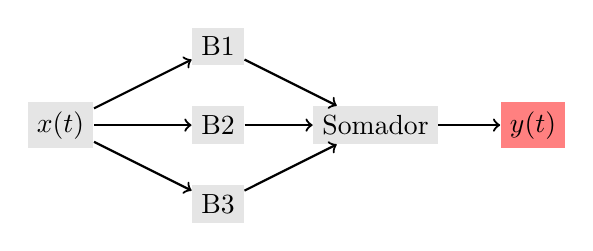
\begin{tikzpicture}
        %======definicao dos blocos==========%
        
            \tikzstyle{vertex}=[rectangle,fill=black!10]
            \tikzstyle{edge}=[->,thick]
            \tikzstyle{vertex_sel}=[rectangle,fill=red!50]
        
        %====================%%=============%  
        
            \node[vertex](A) at (0,0) {$x(t)$};
            \node[vertex](B) at (2,1) {B1};
            \node[vertex](C) at (2,0) {B2};
            \node[vertex](D) at (2,-1) {B3};
            \node[vertex](E) at (4,0) {Somador};
            \node[vertex_sel](F) at (6,0) {$y(t)$};
        
            \draw[edge](A) -- (C);
            \draw[edge](A) -- (B);
            \draw[edge](A) -- (D);
            \draw[edge](D) -- (E);
            \draw[edge](C) -- (E);
            \draw[edge](B) -- (E);
            \draw[edge](E) -- (F);
        \end{tikzpicture}
    \caption{Diagrama de blocos de uma EDO.}
    \label{fig:diagrama_edo}
\end{figure}


O bloco B1 está derivando o sinal de entrada $x(t)$, logo precisaremos utilizar um AmpOp Diferenciador configurando-o para ter um ganho de 5 que é o valor multiplicando o $x'$. Porém, devido aos valores comerciais de um capacitor, ajustou-se para um ganho de 500 que será diminuído mais para frente. Utilizando um $R=500\ohm$ e $C=1F$, tem-se:

\begin{minipage}{.5\textwidth}
    \begin{figure}[H]

        \centering
        
        \begin{circuitikz}[line width = .5pt, scale = .8, transform shape]
            \draw
                (0,0) node [op amp] (opamp) {}
            
            (opamp.-) to [short] ($(opamp.-)+(0,1)$) to [C, l_= C]  ($(opamp.-)+(-2.8,1)$) to [short, -o] ($(opamp.-)+(-3,1)$) node [left]{$V_{in}(t)$}
            (opamp.-) to [short, -*] ($(opamp.-)+(0,1)$)
            to [R, l^=R] ($(opamp.-)+(2,1)$) -| (opamp.out) to [short, *-o] ($(opamp.out)+(1,0)$)
            node [right] {$V_{out}(t)$}
    
            (opamp.+) to [short] ($(opamp.+)+(0,-1)$) node [ground]{}		
            ;
            
            
        \end{circuitikz}
        \caption{Circuito Diferenciador}
        \label{fig:diff_sim}
    \end{figure}
\end{minipage}
\begin{minipage}{.5\textwidth}
    \calc{
        V_{outB1}=-RC\dfrac{dx}{dt}\\
        V_{outB1}=-500\cdot 1 \cdot \dfrac{dx}{dt}\\
        V_{outB1}=-500x'
    }
    
\end{minipage}

No Bloco B2 podemos utilizar um AmpOp Inversor
configurando-o para ter um ganho de 2 que é o
valor multiplicando $x$ nesse bloco. Utilizando um
$R_1=20k\ohm$ e $R_2=10k\ohm$, tem-se:

\begin{minipage}{.5\textwidth}
    
    \begin{figure}[H]
        
        \begin{adjustbox}{width=.7\textwidth}
            \centering
            \begin{circuitikz}[line width=.5pt]
                \draw
                (0, 0) node[op amp] (opamp) {}
                (opamp.-) to[R , l^= $R_1$,-o] (-4, 0.5)node [left]{$V_1$}
                (opamp.-) |- (-1, 2) to[R, l= $R_2$] (1, 2) -| (opamp.out)
                to [short, -o] ($(opamp.out) + (.5,0)$)
                ($(opamp.out) + (.5,0)$) node [right] {$V_o$}
        
        (opamp.+)to [short] ($(opamp.+)+(0,-1)$) node [ground] {}
        
        ;
        
                \draw  (opamp.-) to[short,*-] ++(0,0);    
                \draw  (opamp.out) to[short,-*] ++(0,0);
                
            \end{circuitikz}
        
        \end{adjustbox}
            \caption{Circuito Inversor}
    \end{figure}

\end{minipage}
\begin{minipage}{.5\textwidth}
    \calc{
        V_{outB2}=-\dfrac{R_2}{R_1}x\\
        V_{outB2}=-\dfrac{20k}{10k}x\\
        V_{outB2}=-2x
    }
    \hfill
\end{minipage}

O Bloco B3 é o mais simples de se implementar.
Como todos os meus blocos até agora deram
valores negativos e na equação todos são positivos,
iremos colocar uma fonte DC de -1V para B3. Dessa
forma, podemos utilizar um AmpOp Somador Inversor
para gerar a equação que queremos. Utilizando um
$R_1=10k\ohm$, $R_2=R_3= R_4=100\ohm$, tem-se:

\begin{minipage}{.5\textwidth}
    \begin{figure}[H]
        \centering
        \begin{adjustbox}{width=.7\textwidth}
            \begin{circuitikz}[line width=.5pt] \draw
            (0,0) node [op amp] {}
            (-4.7,1.5) node [right] {$V_1$}
            (-4.7,.5) node [right] {$V_2$}
            (-4.7,-.5) node [right] {$V_3$}
            (-4, 1.5)	to [R, l=$R_1$,  o-] (-2,1.5)
                to [short] (-2,-.5)
            (-4, .5)	to [R, l=$R_3$, o-] (-2,.5)
            (-4, -.5)	to [R, l=$R_4$, o-] (-2,-.5)	
                to [short, -*] (-2,0.5)
                to [short, -*] (opamp.-)
                
            (opamp.+) to [short] ($(opamp.+) + (0, -1.5)$) node [ground]{}
                
            (opamp.-) |- (-1,2) to [R, l=$R_2$] (1,2) -| (opamp.out)
                to [short, *-o] ($(opamp.out) + (1,0)$) node [right] {$V_o$}
            ;    
            
                \end{circuitikz}
            \end{adjustbox}
            \caption{Circuito Somador.}
    \end{figure}
\end{minipage}
\begin{minipage}{.5\textwidth}
    \calc{
        y(t)=-\left(\dfrac{V_{outB1}}{R_1}+\dfrac{V_{outB2}}{R_3}+ \dfrac{V_{outB3}}{R_4}\right)R_2\\
        y(t)=-\left(\dfrac{-500x'}{R_1}+\dfrac{-2x}{R_3}+\dfrac{-1}{R_4}\right)\\
        y(t)=\left(\dfrac{500x'}{10k}+\dfrac{2x}{100}+\dfrac{1}{100}\right)100\\
        y(t)=5x'+2x+1
        }
\end{minipage}

Com isso, conseguimos montar o diagrama de blocos
que gera nossa equação inicial. Agora, vamos
montar a simulação desse circuito no QUCS.

\subsubsection{Simulação de um circuito de Resolução de EDOs}

\begin{itemize}
    \item Abra um novo esquemático.
\end{itemize}

\figura{.3}{imagens/EDO/new}

\begin{itemize}
    \item Na aba Componentes, vá em componentes nãolineares e coloque três Amplificadores Operacionais.
    Vá em componentes agrupados e coloque sete
    resistores e um capacitor.
\end{itemize}

\begin{figure}[H]
    \subfiguras{.2}{1}{imagens/EDO/res_cap}{}{}
    \subfiguras{.2}{1}{imagens/EDO/ampop}{}{}
\end{figure}

\begin{itemize}
    \item  Monte o AmpOp Diferenciador. Conecte os
    componentes sem esquecer da referência do terra e
    ajuste seus valores para os pedidos no exercício.
\end{itemize}

\figuras{.45}{imagens/EDO/diff}{Circuito diferenciador referente ao bloco B1.}{}

\begin{itemize}
    \item Monte o AmpOp Inversor. Conecte os componentes
    sem esquecer da referência do terra e ajuste seus
    valores para os pedidos no exercício.
\end{itemize}

\figuras{.45}{imagens/EDO/inv}{Circuito inversor referente ao bloco B2.}{}

\begin{itemize}
    \item Monte o AmpOp Somador Inversor. Conecte os
    componentes sem esquecer da referência do terra e
    ajuste seus valores para os pedidos no exercício.
    Nomeie a saída.
\end{itemize}

\figuras{.45}{imagens/EDO/sum}{Circuito somador inversor referente ao bloco B3.}{}

\begin{itemize}
    \item Vá em Fontes e coloque uma fonte de tensão
    retangular e duas fontes DC. Vá em Ponteiras e
    coloque uma ponteira de tensão.
\end{itemize}

\begin{figure}[H]

    \subfiguras{.2}{1}{imagens/EDO/rect_source}{}{}
    \subfiguras{.2}{1}{imagens/EDO/dc_source}{}{}
    \subfiguras{.2}{1}{imagens/EDO/probe}{}{}

\end{figure}

\begin{itemize}
    \item Queremos uma onda quadrada com $V_{pp}=2V$, logo U
    deve ser 2V. $TH$ e $TL$ devem ser metade do período,
    logo 0,5. $T_r$ e $T_f$ devem zero.
\end{itemize}

\figuras{.5}{imagens/EDO/edit_rect}{Parâmetros para a fonte de tenão retangular.}{}

\begin{itemize}
    \item Para deslocar a onda na metade da amplitude e
    colocar para ela variar entre +1V e –1V, será utilizada
    uma fonte DC de -1V. Conecte os componentes sem
    esquecer da referência do terra e ajuste seus valores
    para os pedidos no exercício.
\end{itemize}

\figuras{.8}{imagens/EDO/circuito}{}{}

\begin{itemize}
    \item Será utilizada a simulação transiente para se
    observar o comportamento do circuito ao longo do
    tempo. E a simulação DC para as fontes DC.
\end{itemize}

\figuras{.25}{imagens/EDO/simulation}{Inserção dos componentes resposáveis pela simulação.}{}

\begin{itemize}
    \item Como o período da onda é de 1ms, coloque tempo
    suficiente para visualizar o comportamento da onda
    e resolução grande o suficiente para gerar a onda.
\end{itemize}

\figura{.45}{imagens/EDO/trans_sim}

\figuras{1}{imagens/EDO/save_sim}{Parâmetros para simulação transiente.}{}

OBS: Se a simulação estiver demorando muito para a conclusão, diminua a variável step de modo que não perca a qualidade de visualização do gráfico.

\begin{itemize}
    \item Vá em Diagramas e insira um plano cartesiano.
    Coloque o valor das tensões x\_t.Vt e y\_t.Vt. Coloque
    y\_t no o eixo da direita.
\end{itemize}


\figuras{.5}{imagens/EDO/graph_edit}{Edição dos eixos do gráfico.}{}

\begin{itemize}
    \item Por fim, temos a seguinte configuração.
\end{itemize}

\figuras{.8}{imagens/EDO/final}{Comportamento esperado pelo exercício.}{}